%!TEX root = ../main.tex
\section{Results and Analysis}
\label{sec:results}

\subsection{End-to-End Bilingual Evaluation}
\label{sec:e2e}

The complete production pipeline (LanguageDetector $\to$ LanguageAwareTokenizer $\to$
RuleEngine $\to$ backbone inference $\to$ LangAwareFusion with per-language fusion
weights and per-class decision thresholds) is evaluated
on full test splits: Vietnamese ViHSD (6,680) and English Davidson (2,478), yielding
9,158 mixed samples.  Key findings:

\begin{itemize}
    \item Per-language backbone accuracy 87.11\% (VI) and 90.84\% (EN); the
          full hybrid pipeline reaches 87.28\% mixed accuracy (87.32\% VI, 87.17\% EN).
    \item Paired bootstrap + exact McNemar show the hybrid change is not
          significant ($\Delta$macro-F1 $-0.0004$, 95\% CI $[-0.0045,+0.0036]$, $p=0.84$;
          McNemar $p=0.17$).
    \item Language detection 94.11\% accuracy on bilingual stream (fallback 5.89\%).
    \item Full pipeline latency 6.14 ms mean (P95 6.66 ms).
\end{itemize}

Vietnamese backbone macro-F1 0.6608 vs English 0.7676 reflect the ViHSD vs
Davidson datasets rather than the systems; the EN backbone reaches higher
macro-F1 because Davidson's OFFENSIVE class is far more prevalent (1,918/2,478
samples) than ViHSD's HATE class (688/6,680).

% Auto-generated from canonical E2E tuned benchmark
\begin{table}[t]
\centering
\small
\caption{Evaluation on the full test splits: backbone-only inference versus the full pipeline (language detection $\to$ routing $\to$ backbone $\to$ fusion). Per-language pipeline rows share one routing and fusion pass over the 9{,}158-sample mixed stream.}
\label{tab:e2e_full_benchmark}
\begin{tabular}{llcccc}
\toprule
\textbf{Mode} & \textbf{Language} & \textbf{Dataset} & \textbf{$N$} & \textbf{Accuracy} & \textbf{Macro-F1} \\
\midrule
\multirow{2}{*}{Backbone only}
  & Vietnamese & ViHSD & 6{,}680 & 0.8713 & 0.6602 \\
  & English & Davidson & 2{,}478 & 0.8717 & 0.7273 \\
\midrule
\multirow{3}{*}{Full pipeline}
  & Vietnamese & ViHSD & 6{,}680 & 0.8732 & 0.6603 \\
  & English & Davidson & 2{,}478 & 0.8717 & 0.7313 \\
  & \textbf{Mixed} & \textbf{Both} & \textbf{9{,}158} & \textbf{0.8728} & \textbf{0.7787} \\
\bottomrule
\end{tabular}
\end{table}

% Auto-generated from canonical E2E tuned benchmark
\begin{table}[t]
\centering
\small
\begin{tabular}{lccccc}
\toprule
\textbf{Dataset} & \textbf{Lang} & \textbf{Domain} & \textbf{Size ($N$)} & \textbf{Latency} & \textbf{ECE} \\
\midrule
ViHSD Test & Vi & Social media & 6{,}680 & 4.60 ms & 0.112 \\
Davidson Test & En & Hate speech & 2{,}478 & 2.34 ms & 0.110 \\
Mixed E2E & Vi+En & Bilingual & 9{,}158 & 6.14 ms (P95 6.66) & 0.078 \\
\bottomrule
\end{tabular}
\caption{Global cross-lingual benchmark on full test splits. The first two rows are backbone-only inference (per-language AI-only argmax); the last row is the full pipeline (routing $+$ backbone $+$ fusion) with serialised latency and fused-score ECE. \textbf{Note:} English HATE F1 (0.453) is lower than Vietnamese (0.610) due to Davidson dataset HATE class imbalance (5.8\% vs ViHSD 10.3\%).}
\label{tab:global_benchmark}
\end{table}

\subsection{Latency and Throughput Profile}
\label{sec:latency}

Per-request latency (serialised run) averages 6.14 ms per comment (routing $\approx$2.15 ms + AI inference $\approx$4.0 ms),
P95 is 6.66 ms (P99 3.07 ms routing tail), so tail latency stays below 7 ms (Table~\ref{tab:latency}).
Per-request percentiles are measured sequentially (each comment runs the full
routing + inference pipeline); the stage P50/P95 values are summed per request,
so the reported total is a conservative upper bound rather than a percentile
of the per-stage latency distribution.
The routing stage alone processes at 464.5 texts/s; the AI inference stage alone
sustains $\approx$250 texts/s; fusion/decision cost is negligible within the routing pass.
Backbone-only throughput is higher (EN: $\approx$409 texts/s, VI: $\approx$198 texts/s) without routing overhead.

\begin{table}[H]
\centering
\caption{Per-request latency breakdown (ms) and throughput over the 9{,}158-sample bilingual test stream (serialised execution). Stage P50/P95 values are summed per request, so the total P95 conservatively sums stage P95s.}
\label{tab:latency}
\begin{tabularx}{\textwidth}{Xcccc}
\toprule
Pipeline Stage & Mean (ms) & P50 (ms) & P95 (ms) & Thr. (texts/s) \\
\midrule
Routing (langID) & 2.15 & 1.93 & 2.67 & 464.5 \\
AI inference (backbone) & 3.99 & --- & --- & $\approx$250 \\
\midrule
\textbf{Total (serialised)} & \textbf{6.14} & --- & \textbf{6.66} & $\approx$163 \\
\bottomrule
\end{tabularx}
\end{table}

End-to-end throughput on a single laptop GPU meets real-time moderation SLAs;
in this run the AI backbone is the dominant latency component.

\begin{figure}[H]
\centering
\resizebox{0.9\textwidth}{!}{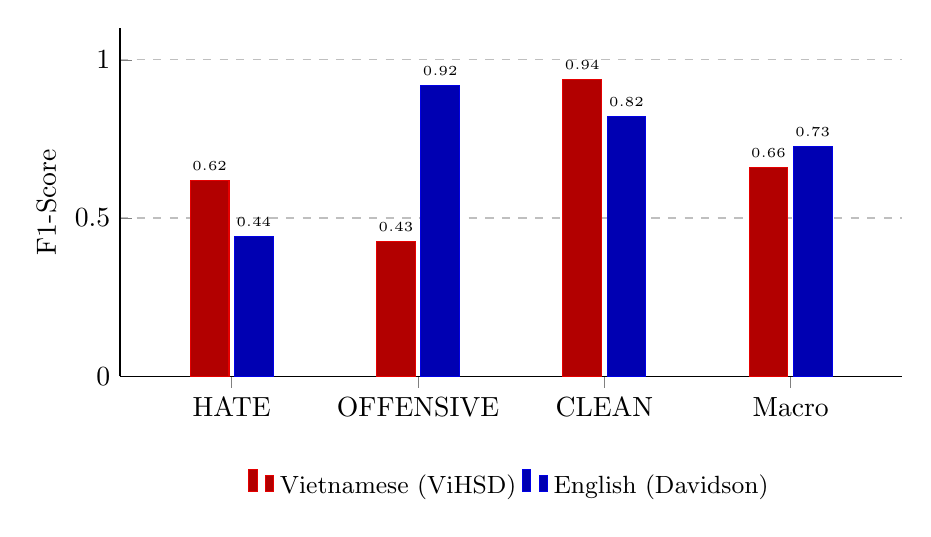
\begin{tikzpicture}
\begin{axis}[
    ybar,
    enlarge x limits=0.2,
    legend style={at={(0.5,-0.25)}, anchor=north, legend columns=-1, draw=none, font=\small},
    ylabel={F1-Score},
    symbolic x coords={HATE, OFFENSIVE, CLEAN, Macro},
    xtick=data,
    nodes near coords,
    nodes near coords align={vertical},
    every node near coord/.append style={font=\tiny\bfseries},
    ymin=0, ymax=1.1,
    width=0.95\textwidth,
    height=6cm,
    bar width=14pt,
    ymajorgrids=true,
    grid style=dashed,
    axis lines*=left,
]
\addplot[fill=red!70!black, draw=red!90!black] coordinates {(HATE,0.6177) (OFFENSIVE,0.4252) (CLEAN,0.9376) (Macro,0.6602)};
\addplot[fill=blue!70!black, draw=blue!90!black] coordinates {(HATE,0.4407) (OFFENSIVE,0.9192) (CLEAN,0.8218) (Macro,0.7273)};
\legend{Vietnamese (ViHSD), English (Davidson)}
\end{axis}
\end{tikzpicture}
}
\caption{F1-score comparison per class and macro-average on the 9,158-sample bilingual test splits (ViHSD 6,680 + Davidson 2,478). Backbone-only inference without routing/fusion.}
\label{fig:f1_comp}
\end{figure}

\subsection{Calibration Diagnostics}
\label{sec:calibration}

Table~\ref{tab:hybrid-calibration} reports calibration diagnostics for AI-only and
Hybrid variants on the bilingual test splits.
While hybrid ECE for ViHSD (0.097) improves over AI-only (0.111), the English
ECE slightly degrades (0.101 $\to$ 0.106) while mean confidence drops from 0.987
to 0.952 (VI) and 0.808 to 0.804 (EN). This indicates that the apparent calibration
gain on ViHSD is a confidence-shrinkage artefact rather than genuine calibration
improvement from rule evidence. We do not claim calibration gains.

\begin{figure}[H]
\centering
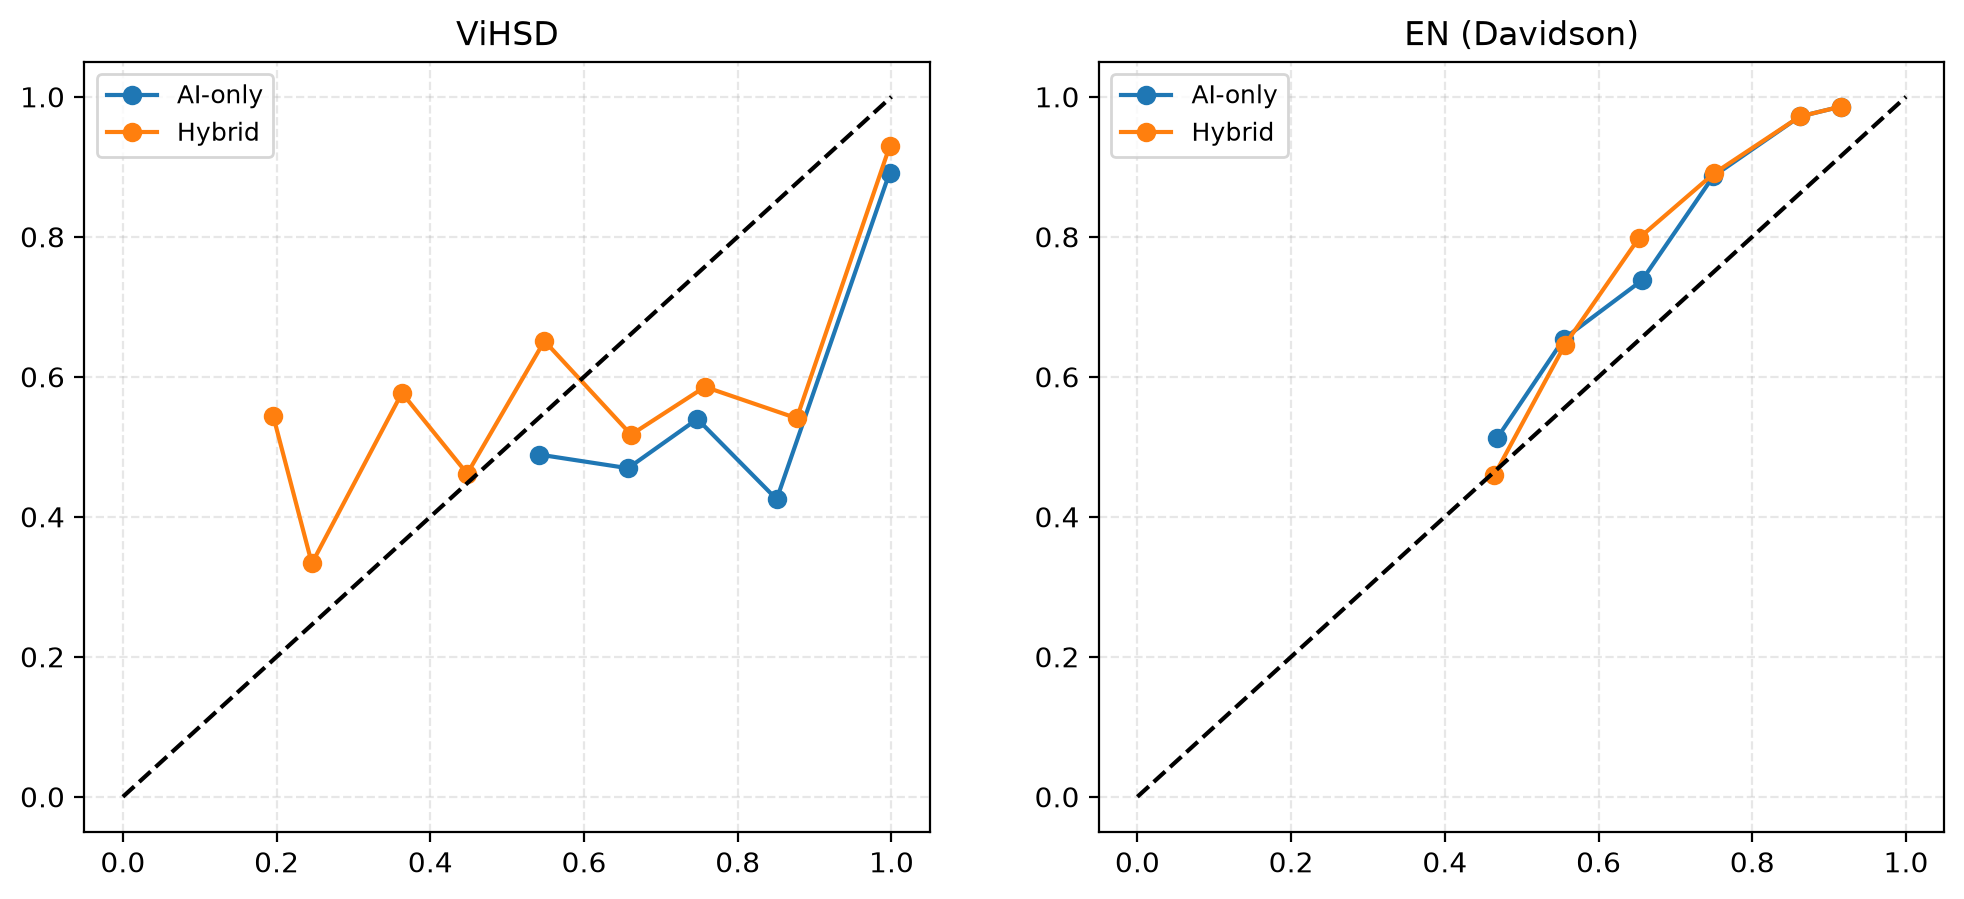
\includegraphics[width=0.8\textwidth]{figures/hybrid_reliability.png}
\caption{Reliability diagram (ECE) comparison between AI-only and Hybrid fusion on the bilingual test sets (left: ViHSD, right: Davidson EN).}
\label{fig:reliability}
\end{figure}

% AUTO-GENERATED BY scripts/57_hybrid_calibration.py - DO NOT EDIT BY HAND
\begin{table}[ht]
\centering
\scriptsize
\setlength{\tabcolsep}{4pt}
\caption{Calibration diagnostics (ECE, Brier, NLL, mean confidence, and macro-F1) for AI-only argmax versus Hybrid on ViHSD test, and full pipeline (fused scores) on 9{,}158 bilingual samples.}
\label{tab:hybrid-calibration}
\begin{tabular}{llcccccc}
\toprule
Variant & Dataset & $n$ & ECE $\downarrow$ & Brier $\downarrow$ & NLL $\downarrow$ & Mean conf. $\uparrow$ & Macro-F1 $\uparrow$ \\
\midrule
AI-only & ViHSD test & 6,680 & 0.112 & 0.240 & 0.825 & 0.984 & 0.660 \\
Hybrid  & ViHSD test & 6,680 & 0.092 & 0.230 & 0.822 & 0.939 & 0.660 \\
Uniform mix ($\alpha=0.70$) & ViHSD test & 6,680 & 0.092 & 0.227 & - & 0.791 & 0.658 \\
\midrule
Mixed E2E (full splits) & ViHSD + Davidson & 9{,}158 & 0.078 & 0.230 & 0.755 & 0.904 & 0.779 \\
\bottomrule
\end{tabular}
\end{table}

\subsection{Robustness to Noisy Vietnamese Surface Forms}
\label{sec:surface}

Teencode, missing diacritics, and deliberate character repetition are pervasive in
user-generated Vietnamese and are the main source of lexical mismatch between the
rule lexicon and incoming text.  Table~\ref{tab:surface-forms} stratifies ViHSD test
performance by surface form using regex detectors over the raw comment, reporting
accuracy, macro-F1, and per-class recall.

Performance degrades most on very long comments ($>500$ chars, macro-F1 0.568)
and on teencode (0.630) and no-diacritics (0.634), which together cover 1,409 test
comments (21.1\%); standard diacritics reach 0.656.  Leet-like repeat characters
perform comparatively well (0.699), indicating that the subword tokenizer absorbs
simple character elongation, whereas teencode and unaccented spellings degrade
accuracy.  HATE recall stays highest on long comments (0.741) but OFFENSIVE recall
collapses to 0.143 there, consistent with mixed hate-plus-offence long posts
being absorbed into the HATE channel.  Short comments ($<20$ chars) obtain the best
accuracy (0.924) and macro-F1 (0.709).

% Auto-generated from outputs/evaluation/analysis/significance_summary.json
% Error stratification for sensitiveai-vi-custom backbone
\begin{table}[ht]
\centering
\scriptsize
\caption{Model performance on challenging surface forms: teencode, no diacritics, repeat characters (leet-like obfuscation), emoji, short text, long text, and standard diacritics on ViHSD test (6,680 samples).}
\label{tab:surface-forms}
\begin{tabular}{lrrrrrrr}
\toprule
\textbf{Category} & \textbf{$N$} & \textbf{Acc} & \textbf{Macro-F1} & \textbf{HATE R} & \textbf{OFF R} & \textbf{CLEAN R} \\
\midrule
Teencode & 1,039 & 0.849 & 0.630 & 0.453 & 0.436 & 0.942 \\
No diacritics & 370 & 0.849 & 0.634 & 0.532 & 0.346 & 0.943 \\
Repeat chars (leet) & 997 & 0.882 & 0.699 & 0.625 & 0.561 & 0.935 \\
Emoji & 974 & 0.912 & 0.616 & 0.426 & 0.367 & 0.972 \\
Very short ($<20$ chars) & 1,852 & 0.924 & 0.709 & 0.553 & 0.534 & 0.972 \\
Very long ($>500$ chars) & 145 & 0.759 & 0.568 & 0.741 & 0.143 & 0.821 \\
With diacritics & 6,114 & 0.876 & 0.656 & 0.532 & 0.418 & 0.955 \\
\midrule
\textbf{Overall (all test)} & \textbf{6,680} & \textbf{0.871} & \textbf{0.661} & -- & -- & -- \\
\bottomrule
\end{tabular}
\end{table}

\subsection{Provenance of Changed Decisions (ViHSD)}
\label{sec:provenance}

On ViHSD, the hybrid changes 64 decisions (39 corrections, 25 regressions, net +14).
Of the 39 corrections, 16 are \hate{} recoveries (7 from \off{}, 9 from \clean{})
and 7 are \clean{} de-flagging cases.  All 16 \hate{} recoveries have a rule firing
with a \hate{} score above the \off{} score, i.e., the rule points in exactly the
corrected direction (median rule \hate{} score 0.765).  All 7 \clean{} de-flagging
cases have a silent rule ($r_H=r_O=0$), so the rule term disappears from the \hate{}
channel and the decision falls back to \clean{}.

The 25 regressions split into 10 rule-driven and 15 threshold-driven cases.
All 10 rule-driven cases (\off{}$\to$\hate{}, \clean{}$\to$\hate{}) have the rule
firing in the \hate{} direction, so fusion trusts lexical \hate{} evidence over the
neural label and the lexicon is wrong about intensity or target.  The 15 threshold-driven
regressions occur when the rule is silent and the fused \hate{} score $0.2\,p_H$
falls below the threshold.
